\apendice{Especificación de diseño}

\section{Introducción}

Las \textit{especificaciones de diseño} juegan un papel crucial en el desarrollo de cualquier proyecto, 
ya que proporcionan una descripción precisa de los \textit{requisitos} y \textit{características} que 
deben cumplir el producto a desarrollar. Estas 
especificaciones son el resultado de un análisis que abarca 
las \textit{necesidades del usuario}, las \textit{limitaciones tecnológicas} y las consideraciones 
de \textit{rendimiento}, \textit{seguridad} y \textit{usabilidad}. Su función es establecer 
los fundamentos para la implementación y permitir que los diseñadores
y desarrolladores trabajen en conjunto en la creación de \textit{soluciones apropiadas}. 
En este sentido, las especificaciones de diseño actúan como una guía esencial para asegurar 
la \textit{calidad} y el \textit{éxito} del proyecto. 

A continuación, se presentan 
las \textit{especificaciones detalladas} que abordan aspectos clave del diseño, tales 
como la arquitectura, las estructuras de datos, el diseño y otros 
elementos críticos necesarios para una \textit{implementación correcta} del sistema.

\section{Diseño de datos}

\subsection{Estructuras de datos}
La información relativa a la red de dependencias de paquetes se almacena en un formato híbrido
que contiene varias estructuras de datos con distintos objetivos:

\begin{itemize}
    \item Almacenar la información concreta de paquetes y dependencias del repositorio, en un formato
          que permita realizar de forma eficiente las operaciones más comunes relacionadas con el objeto
          de la biblioteca.

    \item Ser capaz de aceptar extensibilidad por si en un determinado momento hubiese que ampliar
          o variar los datos que almacenamos.
\end{itemize}
\

De esta forma, representamos cada paquete mediante una estructura de datos específica para
contener los atributos que deseamos representar. La red de dependencias queda representada
como un diccionario de paquetes. Esta representación permite acceder a un paquete de forma
eficiente, lo cual resulta importante para el correcto funcionamiento de la herramienta.

\subsection{Datos de entrada}

Podemos construir la red de dependencias a través de un fichero CSV que represente la lista
de enlaces. Los paquetes se pueden reconstruir a partir de una estructura tipo diccionario
con los atributos implementados. Las listas de paquetes se dan en formato lista de objetos
paquete.

Un problema que se ve es la redundancia de los nombres de nodos, pero realmente es necesario
si queremos almacenar datos más concretos sobre la relación de dependencia, como la versión
concreta de una dependencia que usa un paquete, etc.

\subsection{Datos de salida}
La red se puede exportar a formato de grafo dirigido de \textit{NetworkX} y también como
un diccionario de listas de dependencias.

La estructura de datos \textit{Paquete} se puede exportar como un diccionario, mientras
que un conjunto de paquetes se exportará como una lista de objetos \textit{paquetes}.

\subsection{Ficheros de entrada}
Podemos emplear un archivo CSV como fuente de datos.

Podemos emplear objetos serializados de tipo \textit{PackageManager}.

\subsection{Ficheros de salida}
Podemos generar ficheros \textit{CSV} con la representación de la red o exportarlo como un dataframe de \textit{Pandas},
lo que nos permite exportarlo a otros formatos como \textit{JSON, HTML, etc}.

También podemos realizar un exportado mediante la serialización del objeto \textit{PackageManager}
como estructura global de persistencia para un repositorio. Este tipo de archivo se le ha dado una
extensión \textit{.olvpm} para poder identificarlo correctamente.

\section{Diseño procedimental}

\subsection{Módulo olivia\_finder.package}

\textit{Package} \ref{fig:package} es uno de los módulos base de \textit{olivia-finder}, cuya funcionalidad radica en
constituir una estructura de datos que contiene la representación del paquete. Está compuesto por
atributos en formato \textit{string} y una lista de dependencias (\textit{lista de objetos paquete}).

\begin{figure}[ht!]
    \centering
    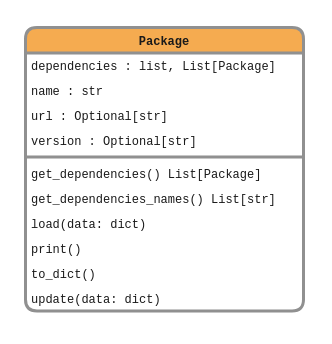
\includegraphics[width=0.4\textwidth]{img/anexos/package.png}
    \caption{Clase Package \textit{package}}
    \label{fig:package}
\end{figure}

En nuestra implementación, los atributos que almacenamos son el nombre, la versión, la URL y las
dependencias. Las principales funcionalidades que implementa son la representación como un
diccionario, la carga a partir de una estructura de tipo diccionario y la enumeración de las
dependencias.

\subsection{Módulo olivia\_finder.package\_manager}

El módulo \textit{Package Manager} \ref{fig:package_manager} es un wrapper de los datos que conforman la red de dependencias de
un repositorio y de la funcionalidad del objeto \textit{DataSource}, que representa la fuente de
datos de un repositorio. Aporta funcionalidades para la carga, obtención y persistencia de los datos.

\begin{figure}[ht!]
    \centering
    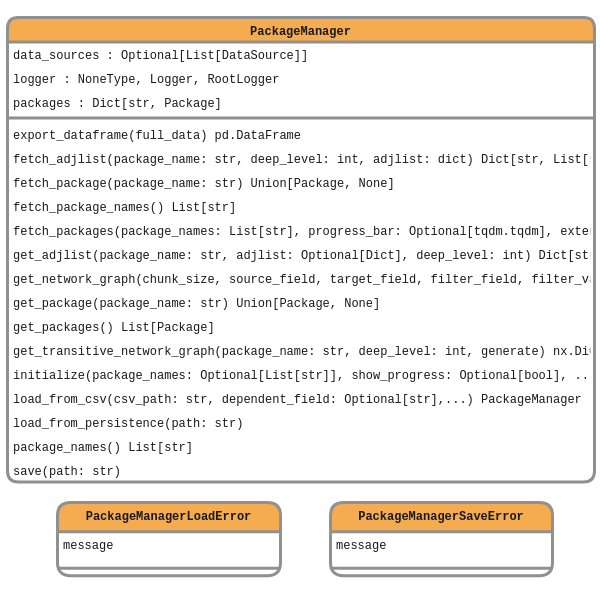
\includegraphics[width=0.8\textwidth]{img/anexos/package_manager.png}
    \caption{Clase \textit{PackageManager}}
    \label{fig:package_manager}
\end{figure}

Para inicializar el objeto, necesitamos pasarle como argumento una lista de los \textit{data sources}
que deseemos usar. Está pensado para tener como mínimo un \textit{data source} principal y una serie
de \textit{data sources} auxiliares opcionales, donde se realizará la búsqueda si no se obtiene un
resultado mediante el principal.

Respecto a la carga de datos en sus estructuras, podemos emplear ficheros de
persistencia \textit{.olvpm} o archivos CSV con la lista de enlaces.

La obtención de datos se puede realizar de forma individual para un paquete o para una lista de
paquetes. Una vez obtenidos los datos, si se desea, se pueden almacenar en la estructura interna
de la clase, que es un diccionario, y recuperarlos desde ahí. Por lo tanto, si queremos usar los
datos directamente desde las estructuras de la clase, primero debemos inicializar los datos.

Una funcionalidad interesante es la obtención de redes de dependencias transitivas a partir de un
paquete y dada una profundidad de búsqueda.

La exportación de los datos se puede representar mediante un objeto diccionario de nodos que
contienen listas de nombres de paquetes, es decir, una lista de adyacencia. El principal formato
de exportación que vamos a tratar son los archivos CSV en formato lista de enlaces, debido a su
naturaleza legible y su integración con OLIVIA. También es interesante su representación como
grafo dirigido de \textit{NetworkX} (\textit{nx.DiGraph}).

La persistencia de los datos se lleva a cabo mediante la serialización del objeto utilizando el
módulo \textit{pickle} de Python, o la generación de archivos CSV de lista de enlaces.

Se incorporan excepciones características para representar los problemas más comunes en un contexto
más descriptivo sobre la actuación de la herramienta.


\subsection{Paquete olivia\_finder.utilities}

El paquete \textit{utilities} \ref{fig:utilities_classes} contiene un conjunto de módulos que implementan funcionalidades de
utilidad para la aplicación, aunque no forman parte central de ella. Está compuesto por los siguientes módulos:

\begin{figure}[ht!]
    \centering
    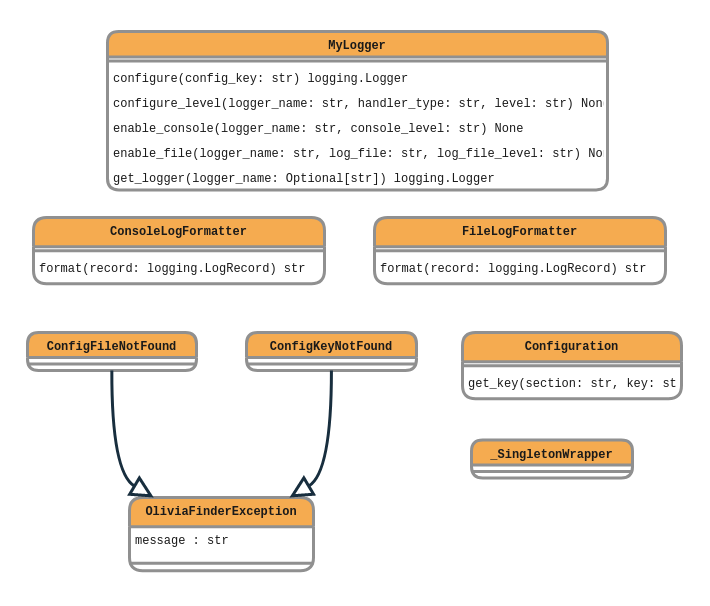
\includegraphics[width=0.8\textwidth]{img/anexos/utilities_classes.png}
    \caption{Diagrama de clases del paquete \textit{utilities}}
    \label{fig:utilities_classes}
\end{figure}



El módulo \textit{config} implementa una funcionalidad para la carga de la configuración
definida en el archivo \textit{config.ini}\footnote{Archivo de configuración de la biblioteca}, donde se especifican las configuraciones necesarias.

El módulo \textit{exception} implementa una excepción genérica para la herramienta, que
puede ser utilizada para capturar y manejar situaciones excepcionales.

El módulo \textit{logger} implementa funcionalidades para llevar un registro de los
eventos ocurridos durante la ejecución de la aplicación.

El módulo \textit{singleton\_decorator} implementa un patrón de diseño singleton basado
en el decorador, que se puede aplicar a cualquier clase para garantizar que sólo se cree una
única instancia de dicha clase.

El módulo \textit{utilities} proporciona algunas funcionalidades concretas y frecuentemente
utilizadas en la aplicación.

\subsection{Paquete olivia\_finder.myrequests}

Este paquete \ref{fig:myrequest_classes} implementa la funcionalidad de realizar \textit{peticiones web} de forma concurrente
y mediante rotación de \textit{proxies} y \textit{user agents} para ocultar la identidad del realizador
de la petición.

\begin{figure}[ht!]
    \centering
    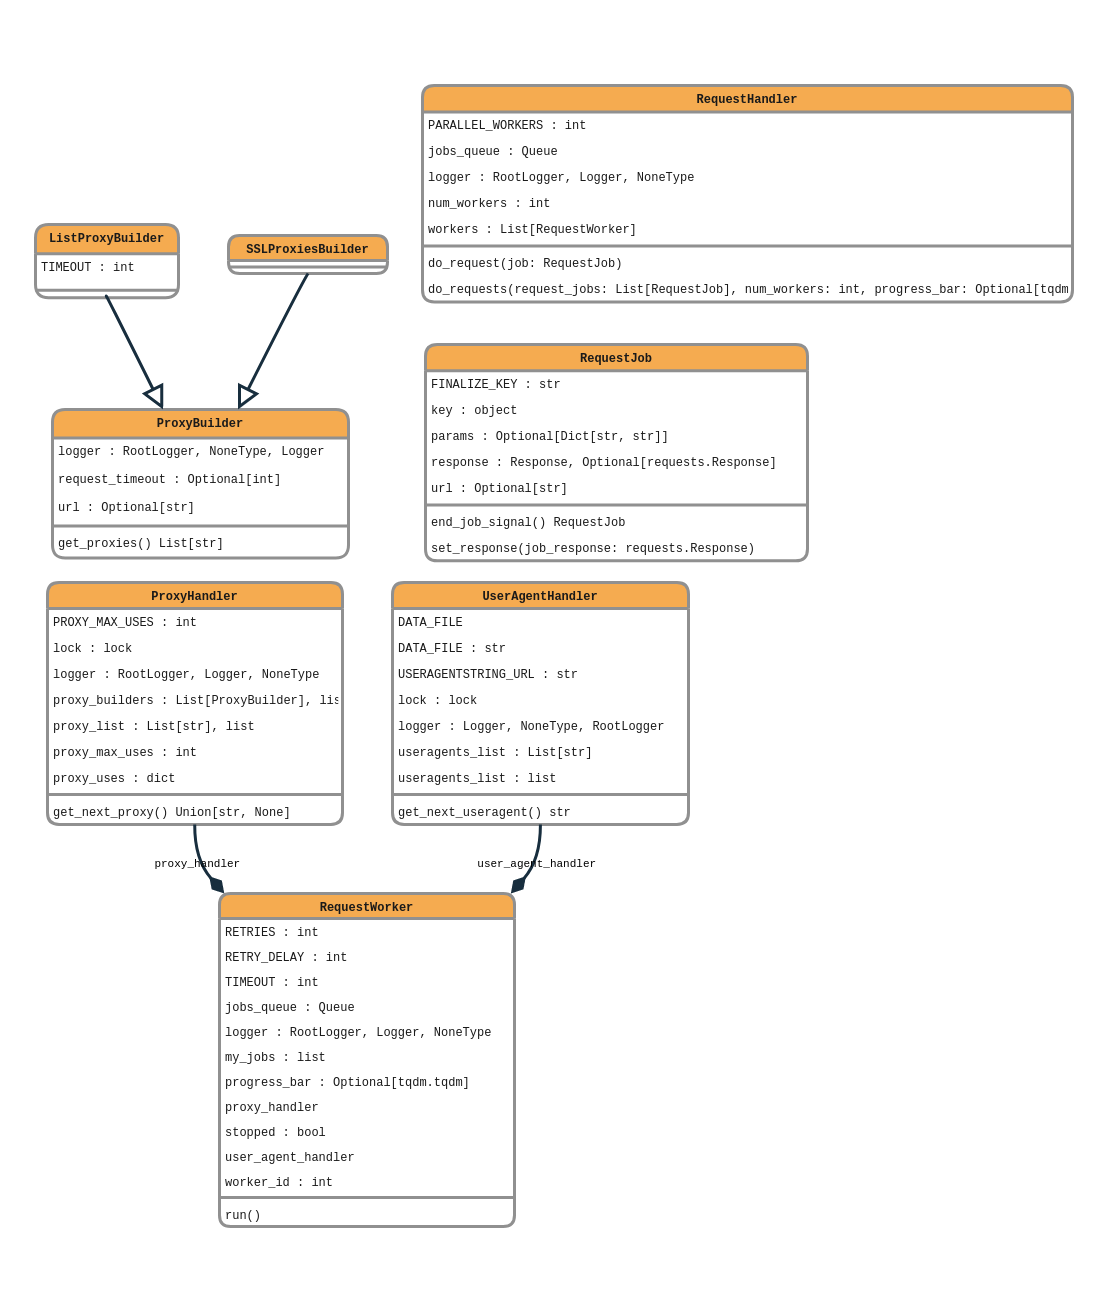
\includegraphics[width=1\textwidth]{img/anexos/myrequests_classes.png}
    \caption{Diagrama de clases del paquete \textit{myrequest}}
    \label{fig:myrequest_classes}
\end{figure}



Está compuesto por los siguientes módulos y paquetes:

El módulo \textit{proxy\_handler} se encarga de gestionar los proxies que se utilizarán para
realizar las peticiones. Lleva un control del número de usos de cada proxy y gestiona su rotación
para evitar la repetición en peticiones concurrentes. Además, obtiene nuevos proxies cuando ha
agotado los existentes. Implementa el patrón de diseño \textit{singleton}.

El paquete \textit{proxy\_builders} implementa la funcionalidad de obtención de una lista de
proxies de Internet. La funcionalidad está descrita en la clase abstracta \textit{ProxyBuilder} del módulo \textit{proxy\_builders},
que se encarga de implementar las funcionalidades comunes y sirve como interfaz para las distintas
clases que implementan \textit{ProxyBuilder}. Estas clases se encuentran en los
módulos \textit{list\_builder} y \textit{ssl\_proxies}.

El módulo \textit{proxy\_builders.list\_builder} se encarga de obtener una lista de proxies almacenada en un
servidor web en formato \textit{txt}.

El módulo \textit{proxy\_builders.ssl\_proxies} realiza la misma función, pero obtiene los datos de los
proxies mediante \textit{web scraping} de un sitio web que ofrece este servicio.

El módulo \textit{useragent\_handler} realiza una función similar al
módulo \textit{proxy\_handler}, pero con los \textit{user agents}. Implementa la obtención a
través de un archivo estático que contiene una lista de \textit{user agents} y también mediante \textit{web scraping} de una página web que contiene un listado. Gestiona la rotación de los \textit{user agents} para evitar su repetición. También implementa el patrón de diseño \textit{singleton}.

El módulo \textit{job} es un \textit{wrapper} de los atributos de una petición web.
Encapsula la URL de destino, los parámetros de la petición y almacena la respuesta del servidor.

El módulo \textit{request\_worker}, que hereda de la clase \textit{Thread}, se encarga de
realizar las peticiones web asignadas a él.

Por último, el módulo \textit{request\_handler} implementa toda la lógica del
paquete \textit{myrequests}. Se encarga de gestionar los trabajos de petición web a realizar y
asignarlos a los \textit{workers}, que se encargan de realizar estas peticiones de forma concurrente.
Recoge los trabajos realizados y los devuelve.

Estos módulos y paquetes en conjunto permiten realizar peticiones web de forma eficiente,
garantizando la anonimización del realizador de la petición mediante el uso de proxies y user
agents rotativos.

\subsection{Paquete olivia\_finder.data\_source}

Este paquete \ref{fig:data_source_classes} implementa la funcionalidad de obtención de datos desde distintas fuentes.

\begin{figure}[ht!]
    \centering
    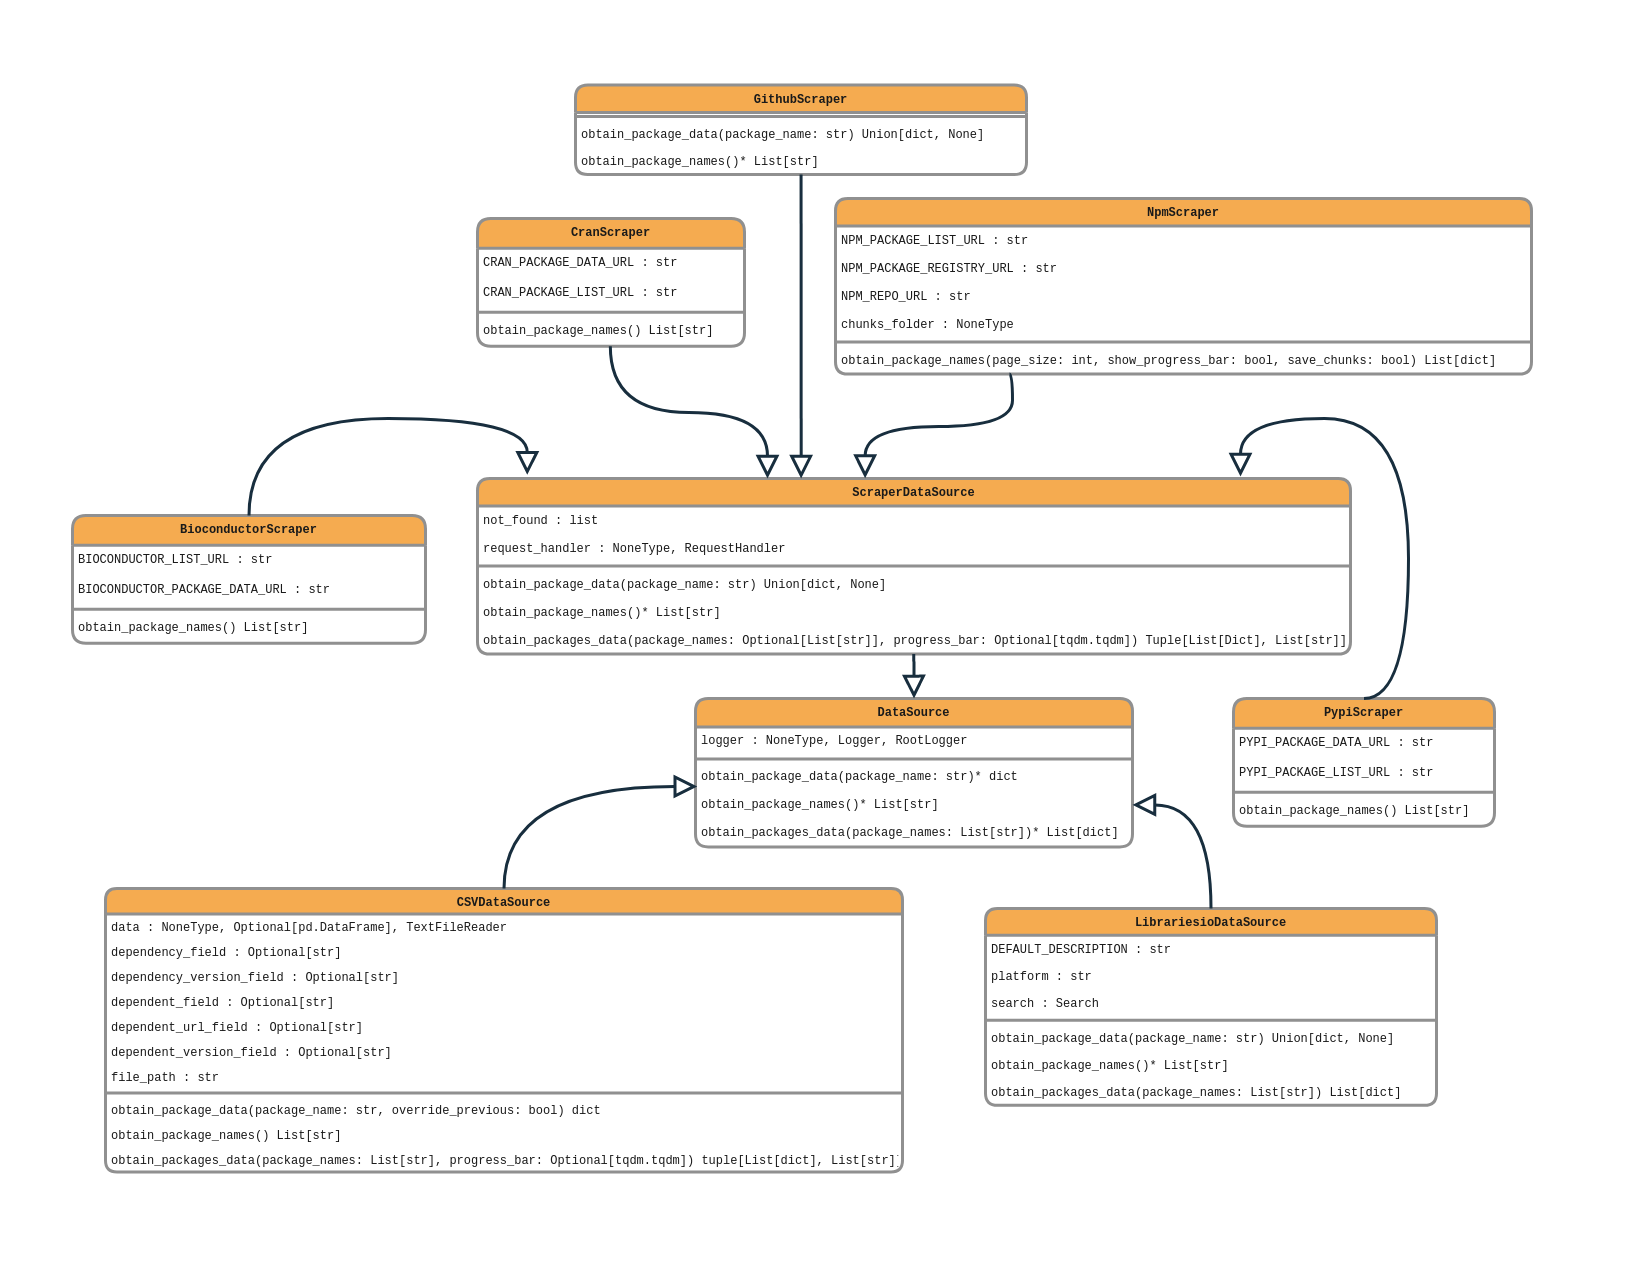
\includegraphics[width=1.2\textwidth]{img/anexos/data_source_classes.png}
    \caption{Diagrama de clases del paquete \textit{data\_source}}
    \label{fig:data_source_classes}
\end{figure}

En primer lugar, tenemos el módulo \textit{data\_source} que implementa una clase abstracta que
sirve como interfaz para las distintas clases de este paquete. Un \textit{data source} debe implementar
la lógica de obtención de una lista de paquetes disponibles y la obtención de los datos de los paquetes.

Tenemos 3 módulos que implementan \textit{DataSource}:

El módulo \textit{data\_source}.\textit{scraper\_ds} implementa la obtención de datos de los paquetes
mediante \textit{web scraping} y proporciona una interfaz para las implementaciones concretas
de \textit{scraper} para los repositorios de software. Las funcionalidades que aporta incluyen
la generación y lanzamiento de trabajos de petición web correspondientes a la obtención de los datos
de los paquetes, así como la recolección de los datos de estas peticiones.

Las implementaciones concretas del módulo \textit{repository\_scrapers}.\textit{scraper\_ds} se encuentran
dentro del subpaquete \textit{repository\_scrapers}, el cual contiene los módulos \textit{repository\_scrapers}.\textit{bioconductor},
\textit{repository\_scrapers}.\textit{cran}, \textit{repository\_scrapers}.\textit{npm}
y \textit{repository\_scrapers}.\textit{pypi}, que realizan la labor descrita para cada uno de
estos repositorios. Además, incluye el módulo \textit{repository\_scrapers}.\textit{github}, que permite
realizar una labor similar a través de la sección \textit{Insights > Dependency graph > Dependencies}, que se puede
habilitar en un repositorio de GitHub.

El módulo \textit{data\_source}.\textit{csv\_ds} proporciona soporte para usar un dataset en formato CSV como fuente de
datos. La funcionalidad que ofrece es similar a la mencionada anteriormente, pero adaptada y optimizada
para este tipo de archivo.

El módulo \textit{data\_source}.\textit{librariesio\_ds} realiza la misma función que los anteriores, pero utiliza la
API de \textit{data\_source}.\textit{Libraries.io}. No todas las funcionalidades han podido ser implementadas en este
módulo, por ejemplo, la lista de paquetes de un repositorio no está soportada. Sin embargo, ofrece
un conjunto de datos más amplio al acceder directamente al conjunto de datos de \textit{Libraries.io}
a través de su API. Para poder utilizar esta funcionalidad, es necesario disponer de una clave de API
de \textit{Libraries.io}.

\section{Diseño arquitectónico}

La arquitectura de la herramienta se basa en un enfoque modular y bien estructurado que permite la
representación y manipulación eficiente de la red de dependencias de paquetes de un repositorio. 

La aplicación se compone de varios módulos y paquetes que trabajan en conjunto para obtener, procesar y persistir los datos.
Cada módulo tiene responsabilidades específicas y se comunica con otros módulos a través de interfaces definidas.
El diseño de datos se centra en la representación de paquetes y dependencias utilizando estructuras de datos
adecuadas, como diccionarios y listas. La aplicación también implementa patrones de diseño, como el patrón singleton,
para garantizar la creación de instancias únicas y la reutilización de recursos. A continuación, se presentarán
los diagramas de clase de cada paquete para proporcionar una visión más detallada de la arquitectura de
la aplicación.


\subsection{Paquete myrequests} \ref{fig:myrequests}

\begin{figure}[ht!]
    \centering
    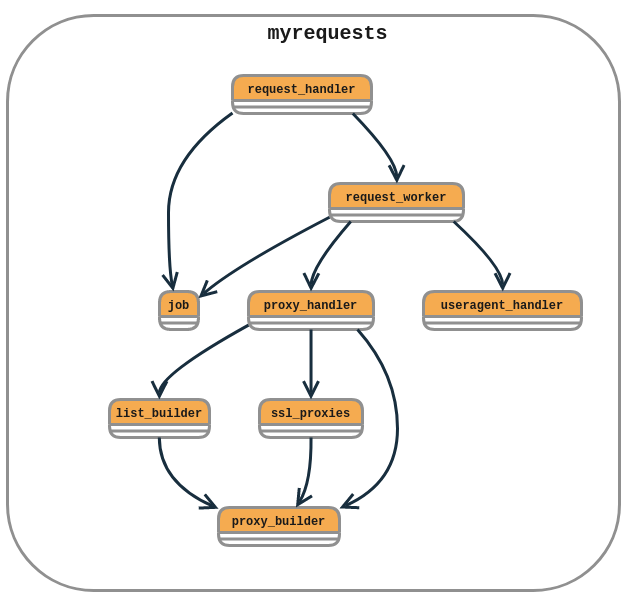
\includegraphics[width=0.6\textwidth]{img/anexos/myrequest.png}
    \caption{Paquete \textit{myrequest}}
    \label{fig:myrequests}
\end{figure}

\subsection{Paquete data\_source} \ref{fig:data_source}

\begin{figure}[ht!]
    \centering
    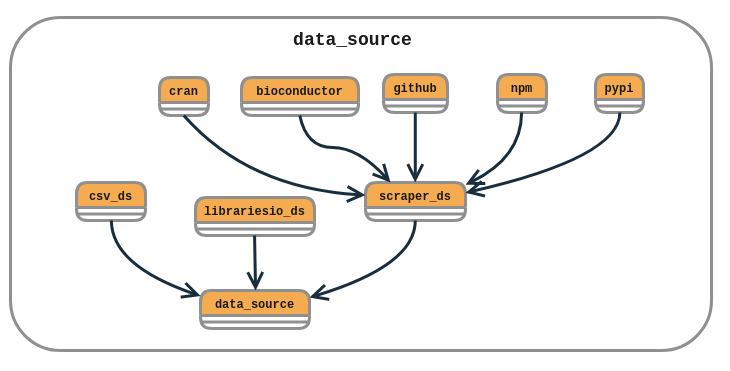
\includegraphics[width=0.8\textwidth]{img/anexos/data_source.png}
    \caption{Paquete \textit{data\_source}}
    \label{fig:data_source}
\end{figure}

\subsection{Paquete utilities} \ref{fig:utilities_package}

\begin{figure}[ht!]
    \centering
    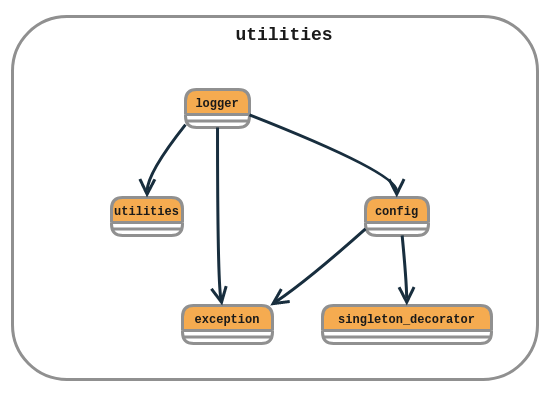
\includegraphics[width=0.6\textwidth]{img/anexos/utilities.png}
    \caption{Paquete \textit{utilities}}
    \label{fig:utilities_package}
\end{figure}